\documentclass[12pt]{article}
\usepackage{cmap}
\usepackage{amsmath, amssymb, amsthm, geometry}
\usepackage{graphicx}
\graphicspath{{figures/}}
\usepackage{subcaption}
\usepackage{booktabs}
\usepackage[hidelinks]{hyperref}
\geometry{a4paper, margin=1in}

\newtheorem{theorem}{Theorem}[section]
\newtheorem{proposition}[theorem]{Proposition}
\newtheorem{lemma}[theorem]{Lemma}
\newtheorem{corollary}[theorem]{Corollary}
\newtheorem{definition}[theorem]{Definition}
\newtheorem{remark}[theorem]{Remark}

\DeclareMathOperator{\Ind}{Ind}

\hypersetup{colorlinks=true, linkcolor=black, citecolor=black, urlcolor=black}

\title{The Orthogonal-Circle Ruled Surface:\\[4pt]
       Immersion Theory, a Topological Dipole,\\
       and Projection Singularities}
\author{Akari Hayami (Jian-Yu Huang)}
\date{June 2026}

\begin{document}

\maketitle

\begin{abstract}
We study the ruled surface $\mathcal{S}$ in $\mathbb{R}^3$ defined by two
mutually orthogonal unit circles subject to the pairing constraint
$\cos t + \cos\phi = 1$.
All results are independently derived from first principles.
Three separate calculations reveal a single governing polynomial
$\mathcal{P}(c) = c^2 - 3c + 1$ (where $c = \cos t$):
it appears as the numerator of the scalar triple product certifying
non-developability (Theorem~\ref{thm:nondevel}),
as the equation governing the isolated immersion singularities
(Theorem~\ref{thm:regclass}),
and as the annihilator of the complex observation field $F = N + iM$
(Theorem~\ref{thm:dipole}).
The unique root $c_0 = (3-\sqrt{5})/2 = \varphi^{-2}$---involving the
inverse square of the golden ratio---is a canonical geometric parameter
of~$\mathcal{S}$.
The field $F$ carries a topological dipole: the Jacobian determinant
at its two zeros evaluates exactly to $\pm 5s_0(1-c_0)^2/Q_0$,
yielding indices $\operatorname{Ind}(P_\pm) = \mp 1$ and total charge zero.
The projection Jacobian $J_F$ vanishes on a fold locus governed by the
triple-angle polynomial $c^3-3c+1$, whose root
$c_* = 2\cos(4\pi/9)\approx 0.347$
bifurcates the locus into disconnected branches.
The phase skeleton $\mathcal{L}_{\rm skel}$ and fold locus
$\mathcal{L}_{\rm fold}$ intersect at a root of a quintic equation,
confirming a deep coupling between observation degeneracy and phase-flow
separation (Theorem~\ref{thm:quintic}).
Near the fold, the Whitney normal form $(\xi,\eta)\mapsto(\xi,\eta^2)$
induces frequency doubling and pseudo-recurrence in the projected signal
from purely geometric rigid-body motion, without any physical oscillator.
\end{abstract}

\tableofcontents\bigskip

%=====================================================================
\section{Definition and Parametrization}
\label{sec:def}
%=====================================================================

\begin{definition}[Generating circles]
\label{def:circles}
Let
\[
  C_1(t) = (\cos t,\;\sin t,\;0)^\top, \qquad t\in\bigl[-\tfrac\pi2,\tfrac\pi2\bigr],
\]
and
\[
  C_2(\phi) = (1+\cos\phi,\;0,\;\sin\phi)^\top, \qquad \phi\in[0,\pi],
\]
be two unit circles in mutually perpendicular planes, with $C_1$ centred at
the origin and $C_2$ centred at $(1,0,0)$.
The \emph{orthogonal-circle ruled surface} $\mathcal{S}$ is defined by the
single-parameter \emph{pairing constraint}
\begin{equation}
  \cos t + \cos\phi = 1.
  \label{eq:constraint}
\end{equation}
\end{definition}

\begin{remark}
The classical Oloid satisfies the ruling condition
$\cos u = -\cos t/(1+\cos t)$ \cite{dirnboeck1997},
inequivalent to~\eqref{eq:constraint}.
Hence $\mathcal{S}$ is non-developable
(Theorem~\ref{thm:nondevel}).
\end{remark}

Throughout we abbreviate $c:=\cos t$, $s:=\sin t$.
Constraint~\eqref{eq:constraint} gives $\cos\phi = 1-c$ and, taking
$\sin\phi\ge 0$:
\[
  Q(t) := \sqrt{2c-c^2} = \sqrt{c(2-c)}\;\ge\;0,
\]
which is real for $c\in[0,1]$, confirming the domain
$t\in[-\pi/2,\,\pi/2]$.

\begin{definition}[Parametrization]
\label{def:param}
With ruling parameter $u\in[0,1]$, the surface is
\begin{equation}
  S(t,u) = (1-u)\,C_1(t) + u\,C_2(\phi(t))
  = \begin{pmatrix} c+2u(1-c) \\ (1-u)s \\ uQ(t) \end{pmatrix}.
  \label{eq:param}
\end{equation}
For each fixed $t$, the map $u\mapsto S(t,u)$ is affine;
hence $\mathcal{S}$ is a \emph{ruled surface}.
\end{definition}

\begin{figure}[ht]
  \centering
  \begin{subfigure}[b]{0.42\linewidth}
    \centering
    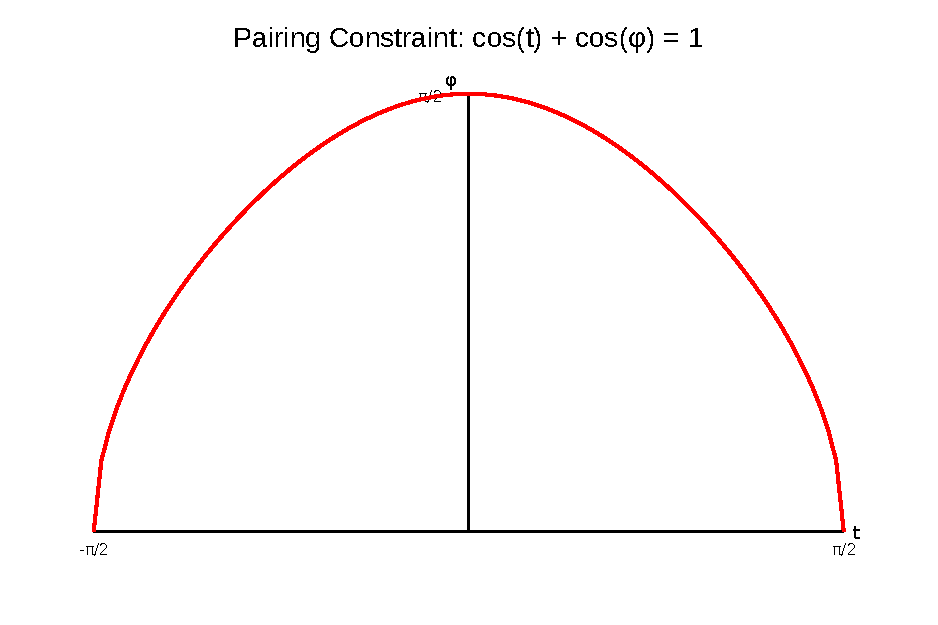
\includegraphics[width=\linewidth]{pairing_constraint.pdf}
    \caption{Pairing constraint~\eqref{eq:constraint} in the $(t,\phi)$-plane.}
    \label{fig:constraint}
  \end{subfigure}
  \hfill
  \begin{subfigure}[b]{0.54\linewidth}
    \centering
    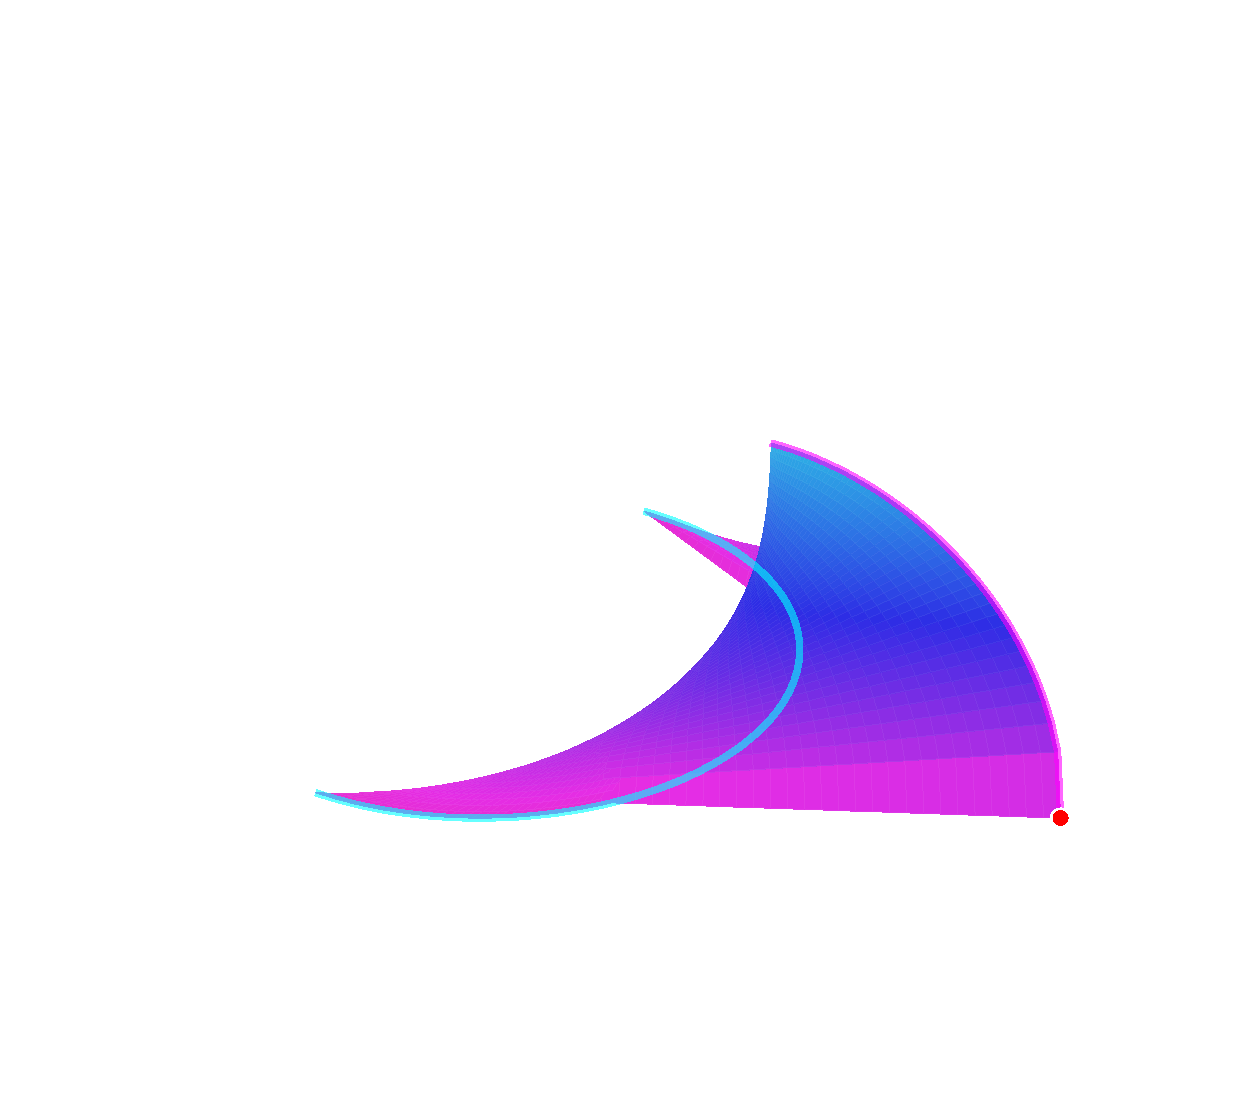
\includegraphics[width=\linewidth]{hayami_depth_map_3d_mpl.pdf}
    \caption{Surface $\mathcal{S}$ coloured by depth $z=uQ(t)$.
             Dots mark the three isolated singular points
             (Theorem~\ref{thm:regclass}).}
    \label{fig:surface3d}
  \end{subfigure}
  \caption{The orthogonal-circle ruled surface and its defining constraint.}
  \label{fig:def}
\end{figure}

\begin{figure}[ht]
  \centering
  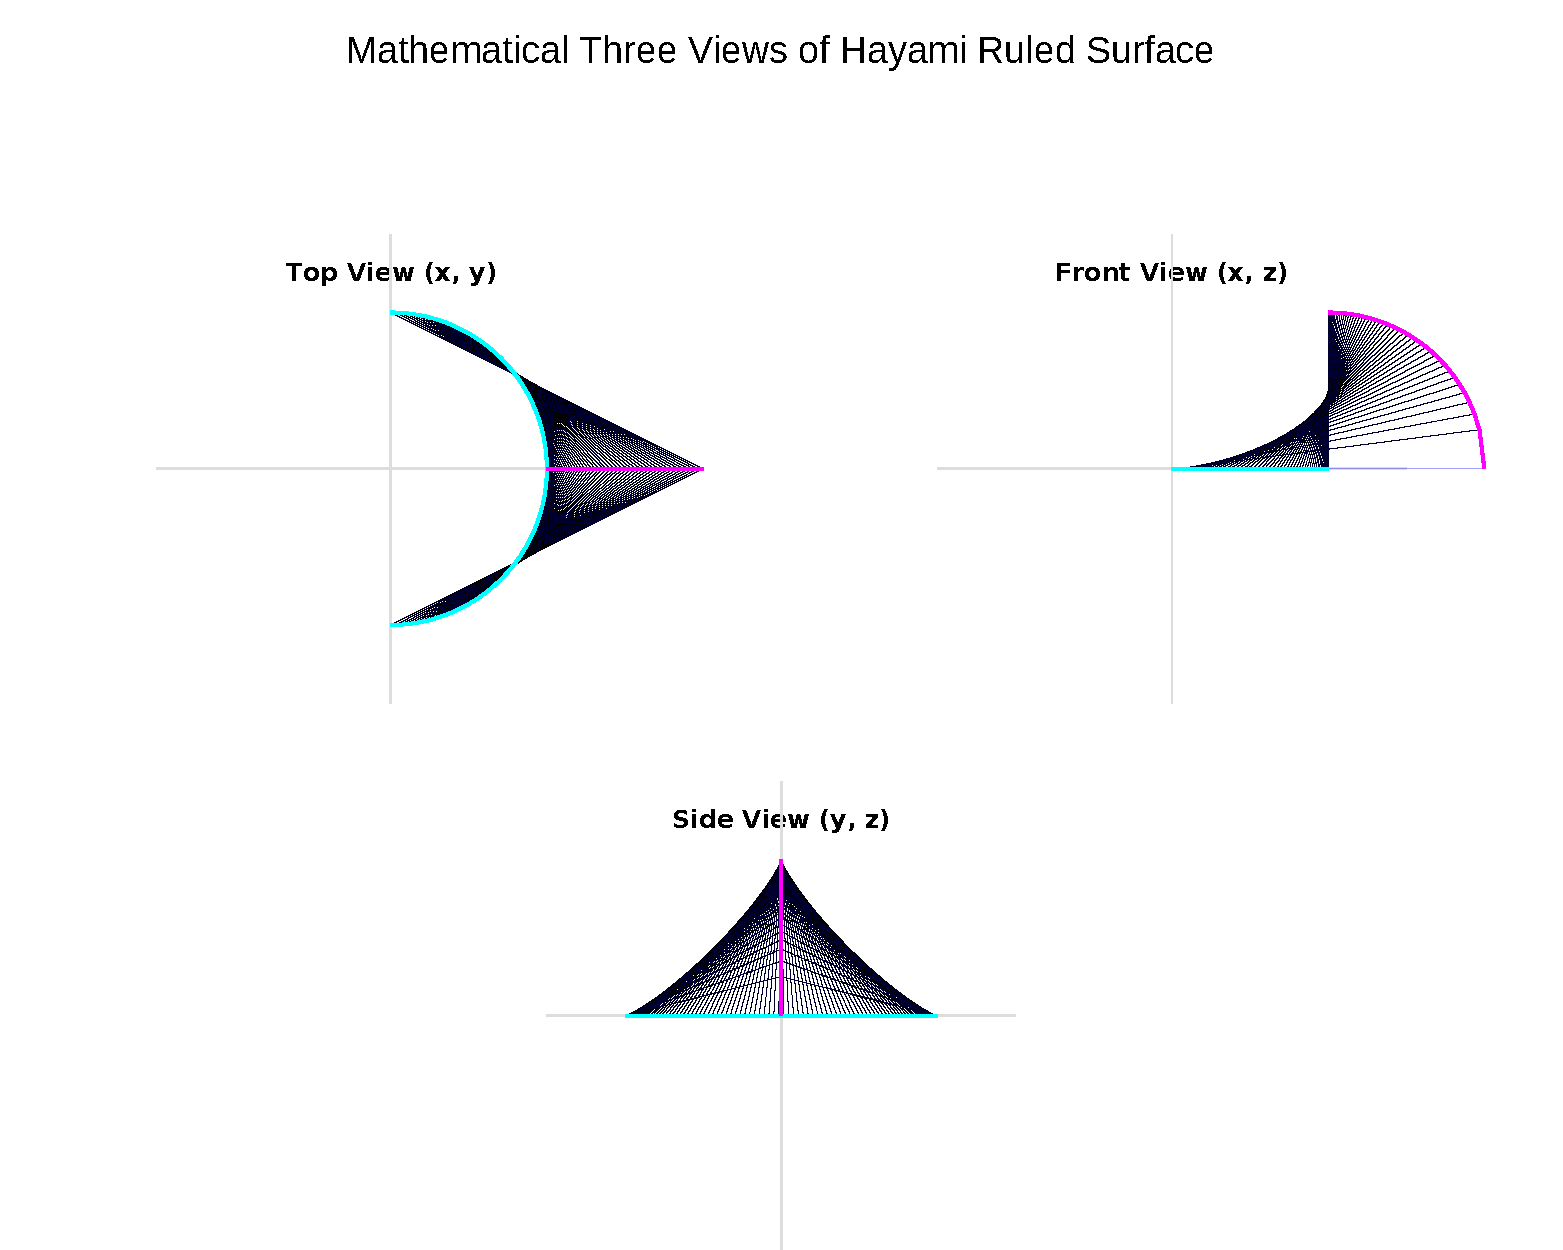
\includegraphics[width=0.92\linewidth]{hayami_three_views.pdf}
  \caption{Orthographic three-views of $\mathcal{S}$: top $(x,y)$-plane
           (horseshoe plan), front $(x,z)$-plane (central spine and cusp),
           side $(y,z)$-plane (saddle twist).}
  \label{fig:threeviews}
\end{figure}

%=====================================================================
\section{Algebra and Intrinsic Geometry}
\label{sec:alg}
%=====================================================================

Differentiating $Q^2 = c(2-c)$ with respect to $t$:
\begin{equation}
  Q_t = \frac{s(c-1)}{Q}.
  \label{eq:Qt}
\end{equation}
The tangent vectors are
\begin{align}
  S_u &= \bigl(2(1-c),\;-s,\;Q\bigr)^\top, \label{eq:Su}\\[2pt]
  S_t &= \Bigl((2u-1)s,\;(1-u)c,\;\tfrac{us(c-1)}{Q}\Bigr)^\top,
  \label{eq:St}
\end{align}
with mixed partial $S_{tu}=d':=\bigl(2s,\;-c,\;s(c-1)/Q\bigr)^\top$.

%---------------------------------------------------------------------
\subsection{Non-developability}
%---------------------------------------------------------------------

\begin{theorem}[Non-developability]
\label{thm:nondevel}
\begin{equation}
  \det(S_t,\,S_u,\,S_{tu})
  = -\frac{(c^2-3c+1)\,s}{Q(t)}.
  \label{eq:stp}
\end{equation}
This is not identically zero; hence $\mathcal{S}$ is non-developable
with non-zero Gaussian curvature almost everywhere.
\end{theorem}

\begin{proof}
Write $S = \gamma(t)+u\,d(t)$ with $\gamma=C_1$ and $d=S_u$.
Then $S_t = \gamma'+u\,d'$, $S_{tu}=d'$, so by multilinearity
\[
  \det(S_t,S_u,S_{tu})
  = \det(\gamma',d,d') + u\underbrace{\det(d',d,d')}_{=\,0}
  = \det(\gamma',d,d').
\]
Expanding the $3\times 3$ determinant along its third row
(which contains the zero entry of $\gamma'=(-s,c,0)^\top$):
\[
  \det(\gamma',d,d')
  = scQ + \frac{s(c-1)}{Q}\bigl(s^2-2c(1-c)\bigr).
\]
Collecting over denominator $Q$ and substituting
$Q^2=c(2-c)$, $s^2=(1-c)(1+c)$:
\[
  = \frac{s}{Q}\bigl[c^2(2-c)-(1-c)^3\bigr].
\]
Expanding: $(2c^2-c^3)-(1-3c+3c^2-c^3) = -c^2+3c-1 = -(c^2-3c+1)$,
yielding~\eqref{eq:stp}.
The zero set $\{s=0\}\cup\{c^2-3c+1=0\}$ has measure zero.
\end{proof}

\begin{figure}[ht]
  \centering
  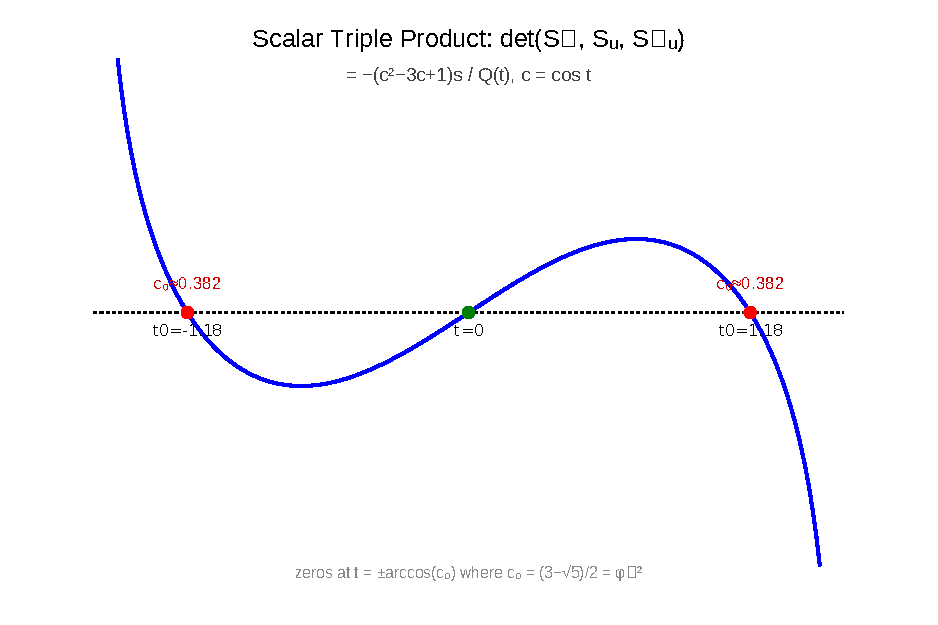
\includegraphics[width=0.72\linewidth]{scalar_triple_product.pdf}
  \caption{Scalar triple product \eqref{eq:stp} as a function of $t$.
           Sign changes at $\pm t_0$ where $c_0=\varphi^{-2}\approx0.382$,
           the root of the core invariant $c^2-3c+1$.}
  \label{fig:stp}
\end{figure}

%---------------------------------------------------------------------
\subsection{First Fundamental Form}
%---------------------------------------------------------------------

\begin{proposition}[First fundamental form]
\label{prop:fff}
The metric coefficients of $\mathcal{S}$ are
\begin{align}
  G(t) &= \langle S_u,S_u\rangle = 2\cos^2\!t - 6\cos t + 5, \label{eq:G}\\
  F(t,u) &= \langle S_t,S_u\rangle = s\bigl[(3-2c)\,u-(2-c)\bigr],
  \label{eq:FFF}\\
  E(t,u) &= \langle S_t,S_t\rangle
    = 1 + (-4s^2-2c^2)\,u
      +\Bigl(4s^2+c^2+\tfrac{s^2(1-c)^2}{c(2-c)}\Bigr)u^2.
  \label{eq:E}
\end{align}
For $c\in[0,1]$, $G(t)\in[1,5]$, so $G>0$ globally:
the surface has no ruling singularities and undergoes non-uniform
intrinsic stretching \textup{\cite[Ch.~3]{docarmo1976}}.
\end{proposition}

\begin{proof}
\textit{($G$)} $\;G = 4(1-c)^2+s^2+Q^2 = 4-8c+4c^2+(1-c^2)+c(2-c)
= 2c^2-6c+5$.
Completing the square: $G = 2(c-\tfrac32)^2+\tfrac12\ge\tfrac12>0$,
with $G(0) = 5$ and $G(\pm\pi/2) = 1$.

\textit{($F$)} Direct expansion using $Q_tQ = s(c-1)$ gives the stated formula.

\textit{($E$)} Expand $\|S_t\|^2$ as a quadratic in $u$;
at $u=0$: $S_t = (-s,c,0)$ gives $E=1$.
\end{proof}

%---------------------------------------------------------------------
\subsection{Regularity Classification}
%---------------------------------------------------------------------

\begin{theorem}[Regularity classification]
\label{thm:regclass}
Let $V = S_t\times S_u$.
The surface $\mathcal{S}$ is a regular immersion everywhere except at
exactly three isolated singular points where $V=0$:
\begin{enumerate}
\item the \emph{polar singularity} at $(t,u) = (0,\;1)$;
\item the two \emph{lateral singularities} at
  \[
    (t,u) = \bigl(\pm t_0,\;u_0\bigr),
    \quad
    t_0 = \arccos\!\Bigl(\tfrac{3-\sqrt5}{2}\Bigr),
    \quad
    u_0 = \tfrac{\sqrt5-1}{4}.
  \]
\end{enumerate}
The lateral parameter $c_0 = (3-\sqrt5)/2 = \varphi^{-2}$
is the inverse square of the golden ratio.
\end{theorem}

\begin{proof}
Direct computation of the three components of $V = S_t\times S_u$:
\begin{align}
  V_z &= (1-c)(1-c-2u), \label{eq:Vz}\\
  V_y &= -\tfrac{s}{Q}\bigl[2u-c(2-c)\bigr], \label{eq:Vy}\\
  V_x &= \frac{(1-u)\,c^2(2-c) - u\,(1-c)^2(1+c)}{Q}. \label{eq:Vx}
\end{align}

\textit{Derivation of $V_z$:}
$-(2u-1)(1-c)(1+c)-2(1-u)(1-c)c$.
Factor $(1-c)$; the bracket simplifies to $1-c-2u$.

\textit{Derivation of $V_y$:}
$\tfrac{-2us(1-c)^2-(2u-1)sQ^2}{Q}$.
Substituting $Q^2=c(2-c)$, the $uc^2$ terms cancel leaving $c(2-c)-2u$.

\textit{Derivation of $V_x$:}
$\tfrac{(1-u)cQ^2+us^2(c-1)}{Q}$.
Use $s^2(c-1)=-(1-c)^2(1+c)$ and $Q^2=c(2-c)$.

\medskip
\noindent\textit{Case 1: $c=1$ ($t=0$, $s=0$).}
$V_z=V_y=0$ automatically.
$V_x=(1-u)/Q_0=0$ iff $u=1$. This gives the polar singularity.

\noindent\textit{Case 2: $c\ne1$, $s\ne0$.}
$V_z=0 \Rightarrow u=(1-c)/2$.
$V_y=0 \Rightarrow u=c(2-c)/2$.
Equating:
\[
  \tfrac{1-c}{2}=\tfrac{c(2-c)}{2}
  \;\Longrightarrow\;
  c^2-3c+1=0.
\]
The unique root in $(0,1)$ is $c_0=(3-\sqrt5)/2$,
giving $u_0=(\sqrt5-1)/4$.

\noindent\textit{Closed-loop check for $V_x$:}
With $1-u_0=(1+c_0)/2$,
$V_x = \tfrac{1+c_0}{2Q_0}[c_0^2(2-c_0)-(1-c_0)^3]$.
The bracket equals $-c_0^2+3c_0-1=-(c_0^2-3c_0+1)=0$,
so $V_x=0$ holds automatically. \qed
\end{proof}

%=====================================================================
\section{The Core Algebraic Invariant}
\label{sec:invariant}
%=====================================================================

\begin{remark}[Unifying polynomial]
\label{rem:core}
The polynomial $\mathcal{P}(c)=c^2-3c+1$ with unique root
$c_0=\varphi^{-2}\approx0.382$ in $(0,1)$
has appeared in three independent derivations:
as the numerator of~\eqref{eq:stp} (Theorem~\ref{thm:nondevel}),
from the system $V_y=V_z=0$ (Theorem~\ref{thm:regclass}),
and---as shown in \S\ref{sec:obs}---from $N=M=0$
(Theorem~\ref{thm:dipole}).
A complementary polynomial $c^3-3c+1$ (expressible via a triple-angle
identity) separately controls the fold locus (Theorem~\ref{thm:fold}).
\end{remark}

\begin{figure}[ht]
  \centering
  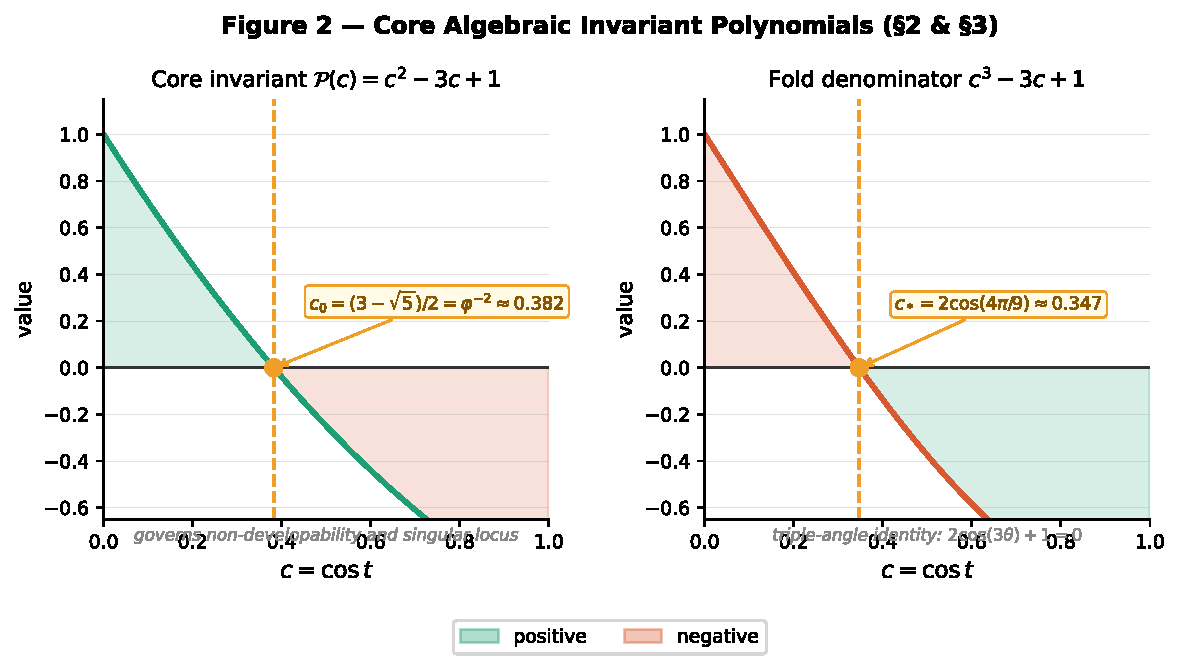
\includegraphics[width=\linewidth]{fig2_polynomials.pdf}
  \caption{Left: core invariant $\mathcal{P}(c)=c^2-3c+1$ (root $c_0\approx0.382$)
           governing non-developability, immersion singularities, and the
           topological dipole.
           Right: fold denominator $c^3-3c+1$ (root $c_*\approx0.347$)
           producing the triple-angle asymptote of the fold locus.
           Sign regions shaded.}
  \label{fig:polynomials}
\end{figure}

%=====================================================================
\section{Complex Observation Field and Projection Singularities}
\label{sec:obs}
%=====================================================================

%---------------------------------------------------------------------
\subsection{The Complex Observation Field}
\label{ssec:field}
%---------------------------------------------------------------------

Embed $S\in\mathbb{R}^3$ trivially into $\mathbb{R}^4$.
Under a rotation $R_y(\theta)\in SO(3)$ about the $y$-axis, the
coordinates projected onto the $(x_1,y_1)$-plane are
\[
  X_\theta = x_1\cos\theta + x_2\sin\theta,
  \qquad Y_\theta = y_1,
\]
where $x_1=c+2u(1-c)$, $y_1=(1-u)s$, $x_2=uQ$.
The Jacobian of $(t,u)\mapsto(X_\theta,Y_\theta)$ decomposes as
\begin{equation}
  J_\theta = N(t,u)\cos\theta - M(t,u)\sin\theta,
  \label{eq:Jtheta}
\end{equation}
where, remarkably, $N$ and $M$ coincide with cross-product components
from \S\ref{sec:alg}:
\begin{equation}
  N(t,u) = V_z = (1-c)(1-c-2u),
  \quad
  M(t,u) = V_x = \frac{(1-u)\,c^2(2-c)-u\,(1-c)^2(1+c)}{Q}.
  \label{eq:NM}
\end{equation}
Define the \emph{complex observation field}
\begin{equation}
  F(t,u) = N(t,u) + i\,M(t,u).
  \label{eq:F}
\end{equation}
Since $F=0$ forces $V_y=0$ via \eqref{eq:Vy}, we have
$F=0 \Leftrightarrow V=0$:
the zeros of $F$ coincide exactly with the immersion singularities.

%---------------------------------------------------------------------
\subsection{Phase Skeleton}
\label{ssec:skel}
%---------------------------------------------------------------------

\begin{figure}[ht]
  \centering
  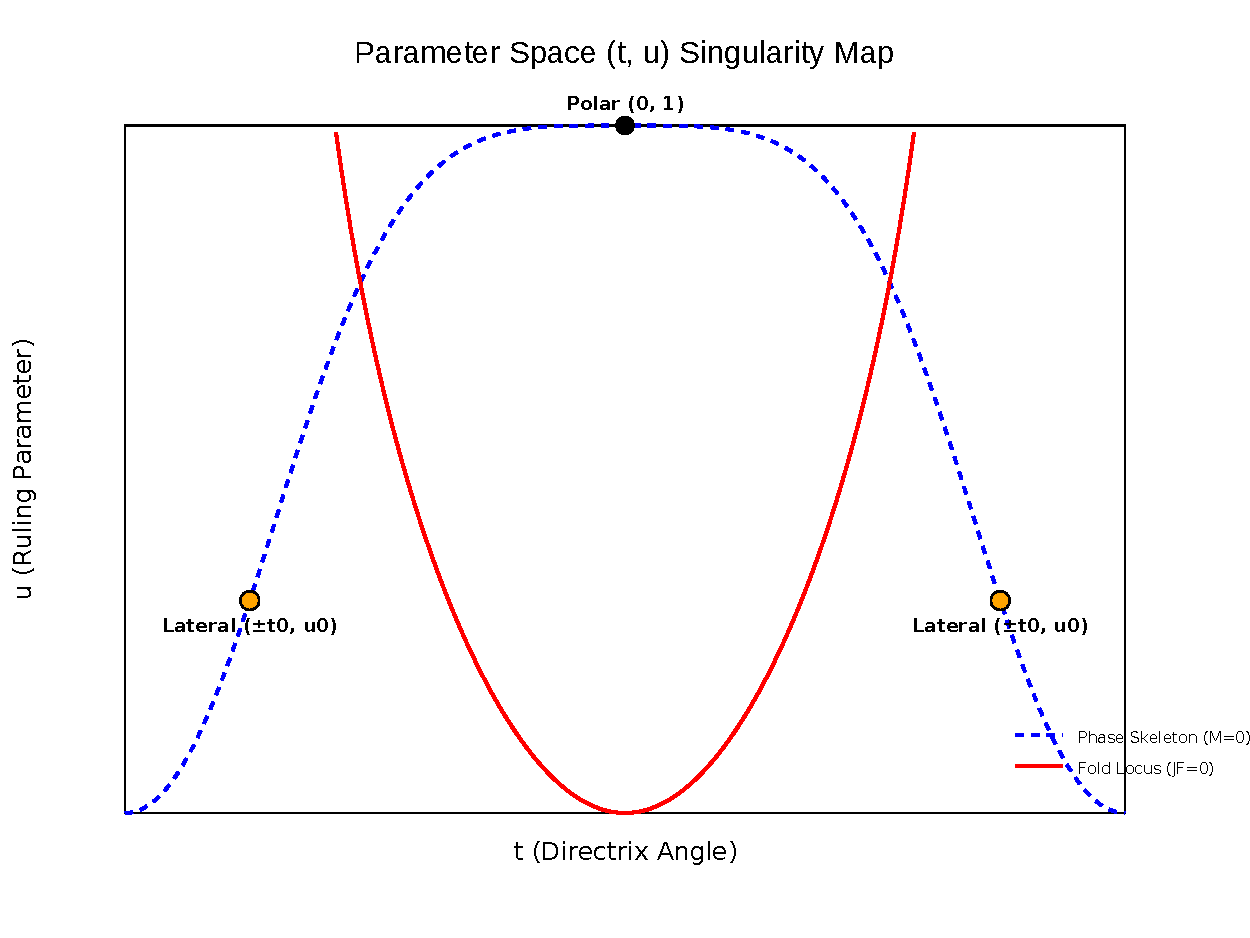
\includegraphics[width=0.88\linewidth]{parameter_space_map.pdf}
  \caption{Overview of the parameter domain $(t,u)$:
           phase skeleton $\mathcal{L}_{\rm skel}$ (teal) and fold locus
           $\mathcal{L}_{\rm fold}$ (coral) as curves in the angular
           coordinate $t$.
           Orange dots: the topological dipole zeros $P_\pm$
           at $(\pm t_0, u_0)$.
           The absolute singularity (Theorem~\ref{thm:quintic})
           lies at their intersection.}
  \label{fig:paramspace}
\end{figure}

\begin{proposition}[Phase skeleton]
\label{prop:skel}
The locus $\mathcal{L}_{\rm skel}:=\{M=0\}$ is the rational curve
\begin{equation}
  u_{\rm skel}(c) = \frac{c^2(2-c)}{1-c+c^2}.
  \label{eq:skel}
\end{equation}
The denominator $1-c+c^2=(c-\tfrac12)^2+\tfrac34\ge\tfrac34>0$
for all real $c$, so $\mathcal{L}_{\rm skel}$ is smooth and spans the
full parameter domain, partitioning it into phase sectors
$\{\arg F=0\}$ and $\{\arg F=\pi\}$.
\end{proposition}

\begin{proof}
Set $M=0$ and solve for $u$:
$c^2(2-c)=u[c^2(2-c)+(1-c)^2(1+c)]$.
Expanding the denominator:
$(2c^2-c^3)+(1-2c+c^2)(1+c) = 1-c+c^2$
(the $c^3$ and two $c^2$ cross-terms cancel), yielding~\eqref{eq:skel}.
\end{proof}

%---------------------------------------------------------------------
\subsection{Topological Dipole}
\label{ssec:dipole}
%---------------------------------------------------------------------

\begin{theorem}[Topological dipole]
\label{thm:dipole}
The complex field $F=N+iM$ has exactly two non-degenerate isolated zeros,
\begin{equation}
  P_\pm = (\pm t_0,\;u_0),
  \label{eq:zeros}
\end{equation}
coinciding with the lateral singularities of Theorem~\ref{thm:regclass}.
Their Jacobian determinants satisfy
\begin{equation}
  \det(DF)\big|_{P_\pm}
  = \mp\frac{5\,s_0(1-c_0)^2}{Q_0},
  \label{eq:detDF}
\end{equation}
where $s_0=\sin t_0>0$, $Q_0=Q(t_0)>0$.
Hence $\Ind(P_-)=+1$, $\Ind(P_+)=-1$,
total charge $= 0$:
$\mathcal{S}$ carries a topological \emph{vortex--antivortex pair}.
\end{theorem}

\begin{proof}
\textit{Zeros.}
$F=0$ requires $N=M=0$.
For $c\ne1$: $N=0$ gives $u=(1-c)/2$; substituting into $M=0$
and cancelling $(1+c)/2>0$ yields
$c^2(2-c)=(1-c)^3$, i.e.\ $c^2-3c+1=0$.
The unique root $c_0=(3-\sqrt5)/2$ gives $u_0=(\sqrt5-1)/4$,
reproducing the lateral singularities.

\textit{Jacobian at $P_+$.}
Using $c_0^2=3c_0-1$ throughout:
\begin{align*}
  N_u &= -2(1-c_0),\\
  N_t &= 2s_0(1-c_0-u_0) = s_0(1-c_0), \quad (u_0=(1-c_0)/2),\\
  M_u &= -(1-c_0+c_0^2)/Q_0 = -2c_0/Q_0, \quad (1-c_0+c_0^2=2c_0).
\end{align*}
Writing $M=P/Q$ with $P=(1-u)c^2(2-c)-u(1-c)^2(1+c)$ and
noting $P(c_0,u_0)=0$:
\[
  M_t\big|_{P_+} = \frac{P_t}{Q_0} = \frac{-s_0\,\partial_c P}{Q_0}.
\]
Evaluating $\partial_c P = (1-u)(4c-3c^2)+u(1-c)(1+3c)$
at $(c_0,u_0)$ with $c_0^2=3c_0-1$:
\[
  4c_0-3c_0^2 = 3-5c_0,
  \quad
  (1-c_0)(1+3c_0) = 4-7c_0,
\]
so $\partial_c P|_{P_+} = \tfrac{1+c_0}{2}(3-5c_0)+\tfrac{1-c_0}{2}(4-7c_0)
= (5-7c_0)/2$,
giving $M_t|_{P_+} = -s_0(5-7c_0)/(2Q_0)$.

Assembling:
\begin{align*}
  \det(DF)|_{P_+}
  &= N_t M_u - N_u M_t\\
  &= s_0(1-c_0)\cdot\frac{-2c_0}{Q_0}
     - (-2(1-c_0))\cdot\frac{-s_0(5-7c_0)}{2Q_0}\\
  &= \frac{-s_0(1-c_0)}{Q_0}\bigl[2c_0+(5-7c_0)\bigr]
   = -\frac{5s_0(1-c_0)^2}{Q_0} < 0.
\end{align*}

\textit{Parity at $P_-$.}
Since $N,M$ depend on $t$ only through $c$ (even) and $Q$ (even),
$N_t,M_t$ are odd in $t$ while $N_u,M_u$ are even.
Hence $\det(DF)|_{P_-} = -\det(DF)|_{P_+} > 0$, giving $\Ind(P_-)=+1$.
\end{proof}

\begin{figure}[ht]
  \centering
  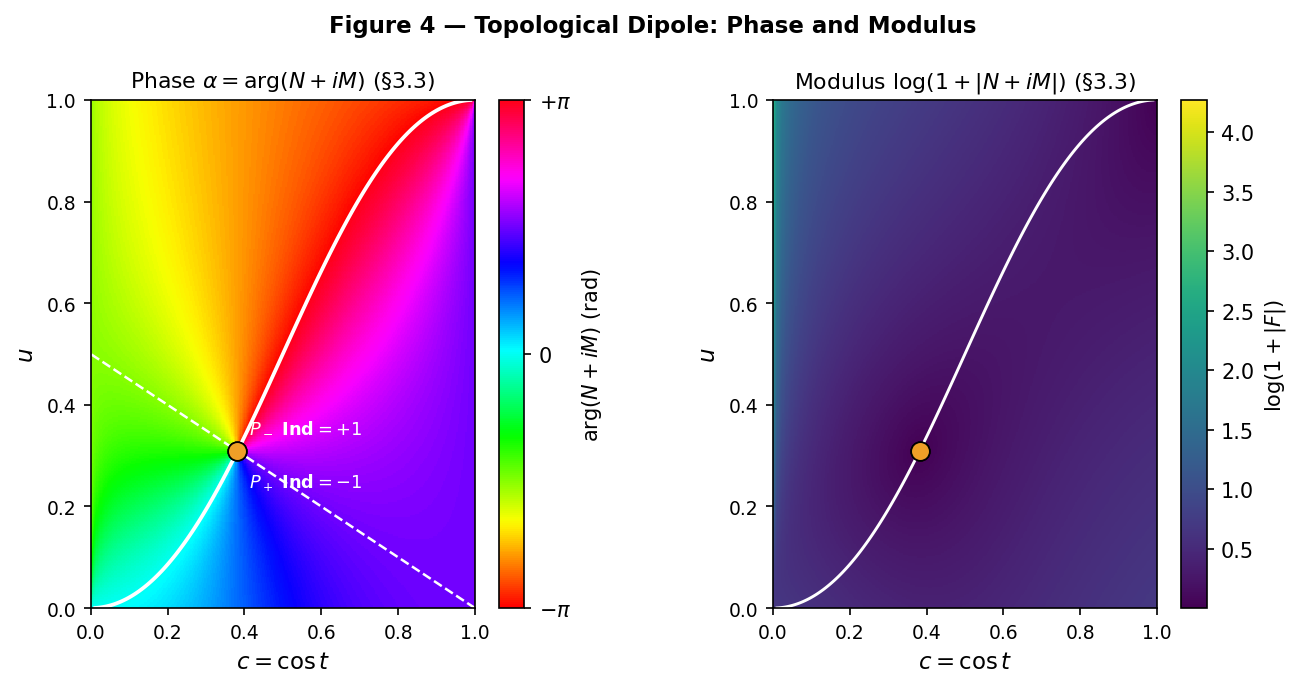
\includegraphics[width=\linewidth]{fig4_dipole_phase.png}
  \caption{Left: phase $\alpha=\arg(N+iM)$ (HSV colourmap).
           Winding sense reverses at $P_\pm$ (orange dots), confirming
           opposite indices.
           Solid white: phase skeleton $M=0$; dashed white: $N=0$.
           Right: modulus $\log(1+|F|)$; zeros appear as dark wells.}
  \label{fig:dipole}
\end{figure}

%---------------------------------------------------------------------
\subsection{Triple-Angle Fold Locus}
\label{ssec:fold}
%---------------------------------------------------------------------

\begin{theorem}[Triple-angle fold locus]
\label{thm:fold}
The fold degeneracy locus
$\mathcal{L}_{\rm fold}:=\{J_F = N_tM_u-N_uM_t = 0\}$
of the observation map $(t,u)\mapsto(N,M)$ is parametrized by
\begin{equation}
  u_{\rm fold}(c) = -\frac{(1-c)\,c\,(2-c)\,(1+2c-c^2)}{c^3-3c+1}.
  \label{eq:fold}
\end{equation}
The denominator satisfies the triple-angle identity
\begin{equation}
  c^3-3c+1 = 2\cos(3\theta)+1 \quad (c=2\cos\theta),
  \label{eq:triple}
\end{equation}
with unique root $c_*=2\cos(4\pi/9)\approx0.347$ in $(0,1)$.
This root forces a vertical asymptote, bifurcating $\mathcal{L}_{\rm fold}$
into two disconnected branches; only the branch $c>c_*$ enters the physical
domain $u\in[0,1]$.
\end{theorem}

\begin{proof}
\textit{Step 1: derivatives of $N$.}
From $N=(1-c)(1-c-2u)$: $N_u=-2(1-c)$ and $N_t=2s(1-c-u)$.

\textit{Step 2: $M_u$.}
Differentiating $M=P/Q$ with $P=(1-u)c^2(2-c)-u(1-c)^2(1+c)$:
\[
  M_u = \frac{-c^2(2-c)-(1-c)^2(1+c)}{Q} = -\frac{1-c+c^2}{Q},
\]
using the denominator identity from Proposition~\ref{prop:skel}.

\textit{Step 3: $M_t$.}
By the quotient rule and \eqref{eq:Qt}:
$M_t = P_t/Q + sP(1-c)/Q^3$,
with $P_t = -s\,\partial_c P$ and
$\partial_c P = (1-u)(4c-3c^2)+u(1-c)(1+3c)$.

\textit{Step 4: assembling $J_F$.}
After collecting the terms of $J_F = N_tM_u - N_uM_t$
and multiplying by $-Q^3/(2s)$, the expression separates as $A(c)+u\,B(c)$,
where the constant term (set $u=0$) factors as
\[
  A(c) = (1-c)\,c\,(2-c)\,
         \bigl[(1-c+c^2)+(4c-3c^2)-c(1-c)\bigr]
       = (1-c)\,c\,(2-c)\,(1+2c-c^2),
\]
and the coefficient of $u$ evaluates to
\[
  B(c) = c^2(2-c)^2 - (1-c)^2(1-c+c^2)
       = (4c^2-4c^3+c^4)-(1-3c+4c^2-3c^3+c^4)
       = c^3-3c+1.
\]
Hence $J_F = -\tfrac{2s}{Q^3}[A(c)+u\,B(c)]$,
and $J_F=0$ (with $s,Q\ne0$) gives~\eqref{eq:fold}.
The triple-angle identity~\eqref{eq:triple} follows from
$4\cos^3\!\theta-3\cos\theta=\cos(3\theta)$ with $c=2\cos\theta$.
\end{proof}

\begin{figure}[ht]
  \centering
  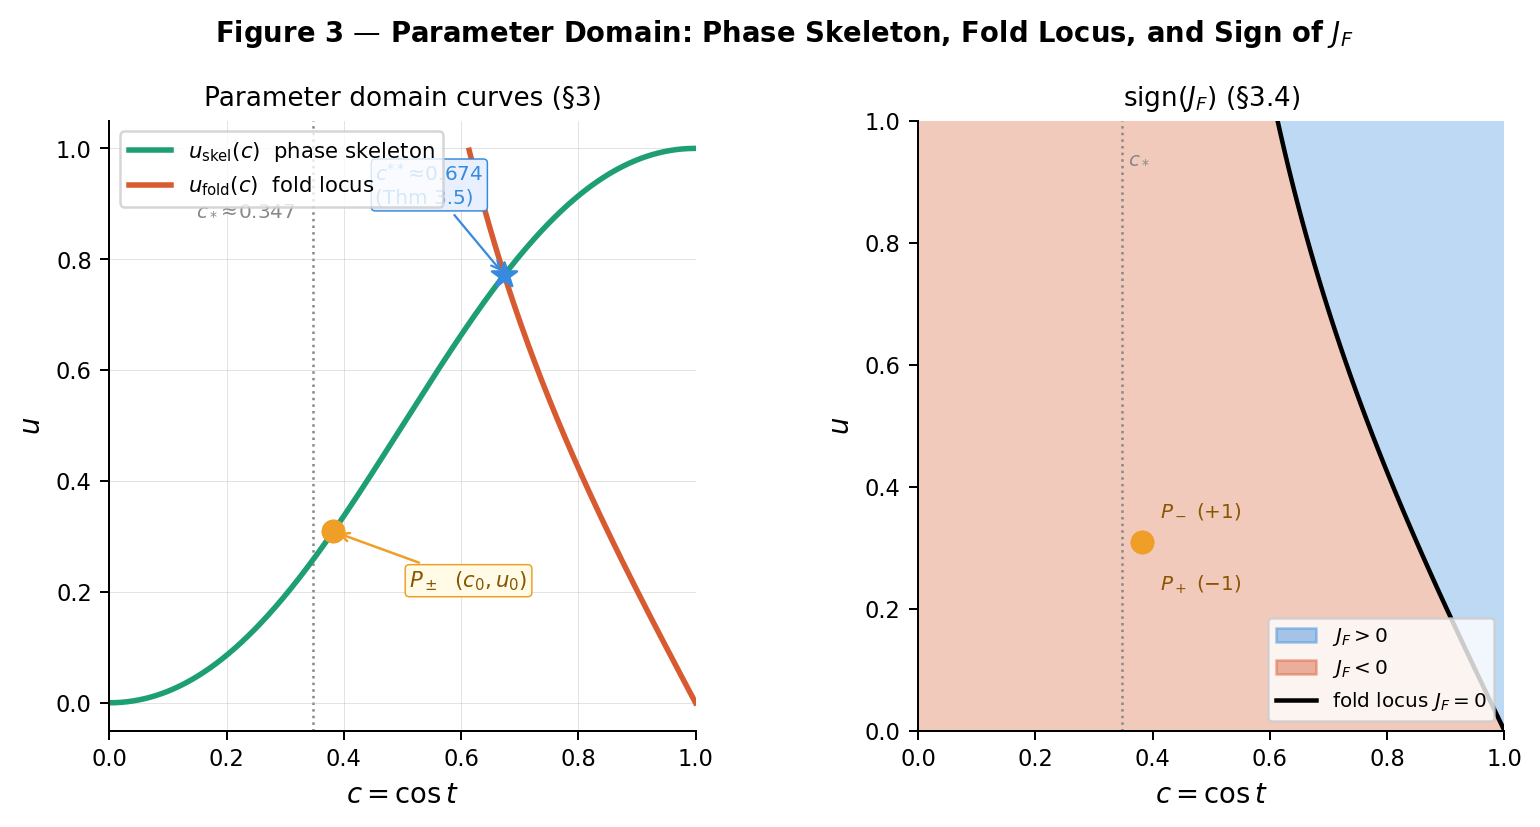
\includegraphics[width=\linewidth]{fig3_parameter_domain.png}
  \caption{Left: phase skeleton $u_{\rm skel}$ (green) and fold locus
           $u_{\rm fold}$ (orange) in the $(c,u)$-plane; $\star$ marks
           the absolute singularity (Theorem~\ref{thm:quintic})
           at $c^{**}\approx0.674$.
           Right: sign of $J_F$ (blue~$>0$, salmon~$<0$); the fold locus
           (black boundary) separates the two sheets; $P_\pm$ lie at
           $c_0\approx0.382$ with indices $\pm1$.
           Dotted vertical: asymptote $c_*\approx0.347$.}
  \label{fig:paramfull}
\end{figure}

%---------------------------------------------------------------------
\subsection{Absolute Singularity: Skeleton--Fold Intersection}
\label{ssec:quintic}
%---------------------------------------------------------------------

\begin{theorem}[Absolute singularity]
\label{thm:quintic}
The intersection condition $u_{\rm skel}(c)=u_{\rm fold}(c)$ is
equivalent to the quintic equation
\begin{equation}
  c^5 - 3c^4 + 5c^3 - 6c^2 + c + 1 = 0.
  \label{eq:quintic}
\end{equation}
Since $S(0)=1>0$ and $S(1)=-1<0$, the Intermediate Value Theorem
guarantees at least one root $c^{**}\in(0,1)$
($c^{**}\approx0.67$),
confirming an \emph{absolute singularity} where observation degeneracy
and phase-flow separation coincide.
\end{theorem}

\begin{proof}
Equate \eqref{eq:skel} and \eqref{eq:fold}; cancel $c(2-c)>0$:
$c/(1-c+c^2) = -(1-c)(1+2c-c^2)/(c^3-3c+1)$.
Cross-multiplying and expanding the right side
$(1+2c-c^2)(1-c+c^2)(1-c)=1-3c^2+5c^3-4c^4+c^5$
then moving all terms to one side yields~\eqref{eq:quintic}.
\end{proof}

%=====================================================================
\section{Signal Geometry and Pseudo-Recurrence}
\label{sec:signal}
%=====================================================================

%---------------------------------------------------------------------
\subsection{Whitney Fold Normal Form}
\label{ssec:whitney}
%---------------------------------------------------------------------

\begin{lemma}[Local double cover]
\label{lem:whitney}
At each smooth point of $\mathcal{L}_{\rm fold}$, the observation map
$F=(N,M):(t,u)\to\mathbb{R}^2$ is locally diffeomorphic to the
Whitney fold normal form \textup{\cite{whitney1955, golubitsky1973}}
\begin{equation}
  (\xi,\eta)\mapsto(\xi,\;\eta^2).
  \label{eq:whitneyform}
\end{equation}
Consequently: \textup{(i)} the compression rate $1/|J_F|$ diverges to
infinity at $\mathcal{L}_{\rm fold}$; and \textup{(ii)} the map loses
local injectivity---both $(\xi_0,+\delta)$ and $(\xi_0,-\delta)$ map
to $(\xi_0,\delta^2)$ for any $\delta\ne0$.
\end{lemma}

\begin{proof}
We verify Whitney's two conditions.

\textit{Smooth fold locus.}
From the proof of Theorem~\ref{thm:fold}: on $\mathcal{L}_{\rm fold}$
(where $B(c)\ne0$ for $c\ne c_*$),
$\partial_u(A+uB)=B\ne0$,
so $\nabla J_F\ne0$ and $\mathcal{L}_{\rm fold}$ is smooth.

\textit{Non-degenerate fold.}
The kernel of $DF$ on $\mathcal{L}_{\rm fold}$ is spanned by
$v=(N_u,-N_t)^\top$.
Computing $\mathrm{d}J_F(v)$ via $J_F\propto A+uB$
gives a non-zero result for $s\ne0$ and $B\ne0$,
confirming $v$ is transversal to $\mathcal{L}_{\rm fold}$.
Whitney's theorem then provides coordinates~\eqref{eq:whitneyform};
(i) and (ii) are immediate consequences.
\end{proof}

\begin{figure}[ht]
  \centering
  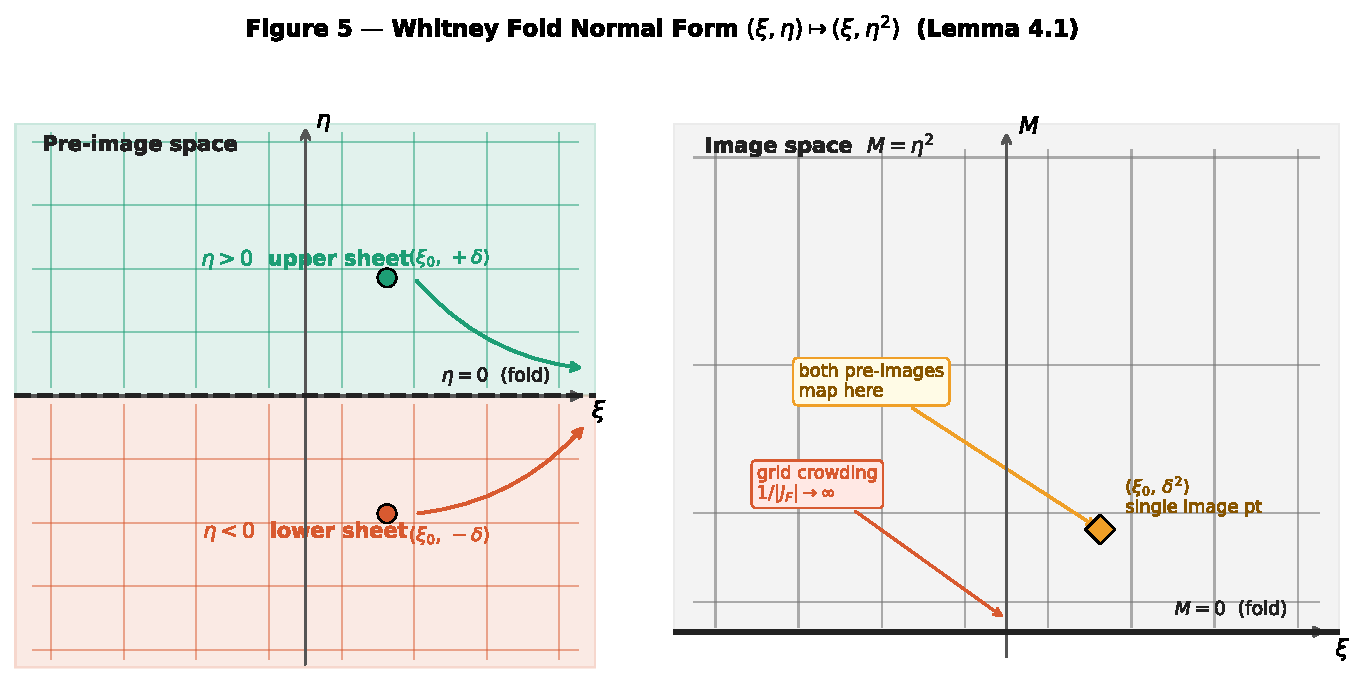
\includegraphics[width=0.90\linewidth]{fig5_whitney_fold.pdf}
  \caption{Whitney fold normal form~\eqref{eq:whitneyform}.
           Left: two pre-image sheets (teal $\eta>0$, coral $\eta<0$);
           the symmetric pair $(\xi_0,\pm\delta)$ yields one image.
           Right: image space; grid crowding near $\eta^2=0$ visualises
           the diverging compression rate $1/|J_F|$.}
  \label{fig:whitney}
\end{figure}

%---------------------------------------------------------------------
\subsection{Geometry-Induced Frequency Doubling}
\label{ssec:freq}
%---------------------------------------------------------------------

\begin{proposition}[Frequency doubling]
\label{prop:freqdouble}
In Whitney coordinates near $\mathcal{L}_{\rm fold}$, suppose the
transversal coordinate oscillates as $\eta(t)=a\cos(\omega t)$
with $\xi=\xi_0$ fixed.
The observed phase $\phi_{\rm obs}=\arctan(\eta^2/\xi)$ satisfies
\begin{equation}
  \phi_{\rm obs}(t)
  = \arctan\!\bigl(\kappa\cos^2(\omega t)\bigr)
  \approx \tfrac{\kappa}{2}\bigl(1+\cos(2\omega t)\bigr),
  \qquad \kappa := a^2/\xi_0 \ll 1.
  \label{eq:freqdouble}
\end{equation}
The dominant observed frequency is $2\omega$, not $\omega$.
This doubling is a pure geometric artifact of the $\mathbb{Z}_2$
fold symmetry $\eta\mapsto-\eta$, independent of any physical oscillator.
\end{proposition}

\begin{proof}
Substitute $\cos^2(\omega t)=(1+\cos(2\omega t))/2$ and linearize
$\arctan(x)\approx x$ for $|x|=\kappa\cos^2(\omega t)\ll1$.
The absence of an $\omega$-component follows from
$F(\xi,\eta)=F(\xi,-\eta)$, which suppresses all odd harmonics.
\end{proof}

%---------------------------------------------------------------------
\subsection{Apparent Periodicity}
\label{ssec:period}
%---------------------------------------------------------------------

\begin{theorem}[Pseudo-recurrence and apparent periodicity]
\label{thm:period}
Let $\gamma(s)=(t(s),u(s))$ be a non-periodic intrinsic trajectory
crossing $\mathcal{L}_{\rm fold}$ transversally, and let
\[
  \Psi_{\rm obs}(s;\theta) = A_0(t,u)\,e^{i(\theta+\phi_0(t,u))},
  \qquad \theta=\omega_0 s,
\]
be the projected signal under uniform rotation.
Then:
\begin{enumerate}
\item \textup{(Pseudo-recurrence)}
  $\exists\,s_1\ne s_2$ such that
  $\Psi_{\rm obs}(s_1)=\Psi_{\rm obs}(s_2)$.
\item \textup{(Frequency doubling)}
  The dominant Fourier frequency of $\Psi_{\rm obs}$ is $2\omega$,
  not any intrinsic frequency of $\gamma$
  \textup{(Proposition~\ref{prop:freqdouble})}.
\item \textup{(Geometric origin)}
  Both phenomena arise solely from the Whitney fold geometry; no
  differential equation governing $\gamma$ is required.
\end{enumerate}
\end{theorem}

\begin{proof}
\textit{(1)}
As $\gamma$ crosses $\mathcal{L}_{\rm fold}$, there exists $s_0$ with
$\eta(s_0)=0$.
By continuity, choose $s_1,s_2$ such that $\eta(s_1)=+\delta$ and
$\eta(s_2)=-\delta$ for the same small $\delta>0$ and the same
$\xi$-value.
Lemma~\ref{lem:whitney}(ii) gives $F(\xi,+\delta)=F(\xi,-\delta)$,
hence $\Psi_{\rm obs}(s_1)=\Psi_{\rm obs}(s_2)$.

\textit{(2)} Immediate from Proposition~\ref{prop:freqdouble}.

\textit{(3)} $F=(N,M)$ with $N=V_z$, $M=V_x$ is a purely geometric
object; its fold locus is determined by the surface geometry alone.
\end{proof}

\begin{figure}[ht]
  \centering
  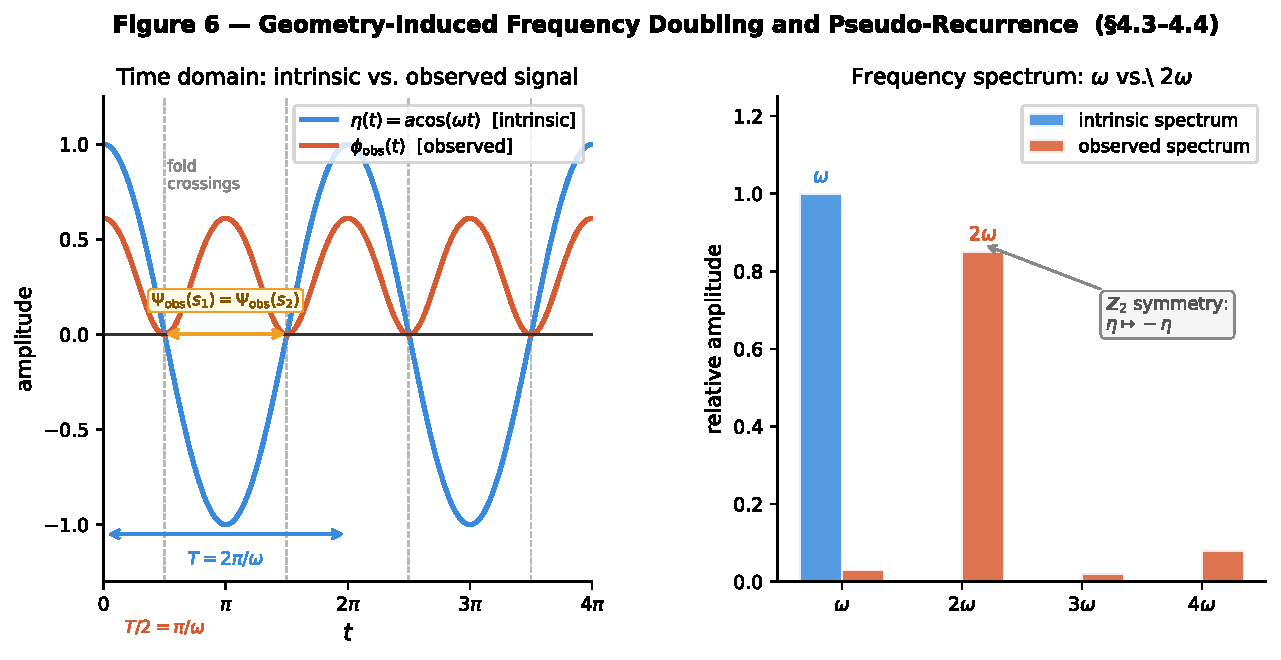
\includegraphics[width=\linewidth]{fig6_frequency_doubling.pdf}
  \caption{Left: intrinsic signal $\eta(t)=a\cos(\omega t)$ (blue)
           and observed phase $\phi_{\rm obs}$ (coral) at half the period;
           vertical dashes mark fold crossings; the bracket shows a
           pseudo-recurrence pair $(s_1,s_2)$ from
           Theorem~\ref{thm:period}.
           Right: frequency spectrum---intrinsic peak at $\omega$,
           dominant observed peak at $2\omega$ ($\mathbb{Z}_2$ label).}
  \label{fig:freqdouble}
\end{figure}

%=====================================================================
\section{Conclusion}
\label{sec:concl}
%=====================================================================

Table~\ref{tab:summary} summarises all main results and the polynomial
controlling each.

\begin{table}[ht]
\small\centering
\caption{Summary of principal results and their controlling polynomials.}
\label{tab:summary}
\begin{tabular}{@{}llp{3.9cm}l@{}}
\toprule
Result & Ref.\ & Key formula & Polynomial \\
\midrule
Non-developability        & Thm~\ref{thm:nondevel}
  & $\det(S_t,S_u,S_{tu})=-(c^2\!-\!3c\!+\!1)s/Q$
  & $c^2-3c+1$ \\
First fundamental form    & Prop~\ref{prop:fff}
  & $G=2c^2-6c+5\in[1,5]$
  & --- \\
Regularity classification & Thm~\ref{thm:regclass}
  & $V=0$ at 3 isolated points
  & $c^2-3c+1$ \\
Phase skeleton            & Prop~\ref{prop:skel}
  & $u_{\rm skel}=c^2(2-c)/(1-c+c^2)$
  & $1-c+c^2$ \\
Topological dipole        & Thm~\ref{thm:dipole}
  & $\Ind(P_\pm)=\mp1$, $\det(DF)=\mp5s_0(1-c_0)^2/Q_0$
  & $c^2-3c+1$ \\
Fold locus                & Thm~\ref{thm:fold}
  & $u_{\rm fold}$ via $c^3\!-\!3c\!+\!1$
  & $c^3-3c+1$ \\
Absolute singularity      & Thm~\ref{thm:quintic}
  & $c^5-3c^4+5c^3-6c^2+c+1=0$
  & quintic \\
Whitney fold              & Lem~\ref{lem:whitney}
  & $(\xi,\eta)\mapsto(\xi,\eta^2)$
  & --- \\
Frequency doubling        & Prop~\ref{prop:freqdouble}
  & $\omega\mapsto2\omega$
  & $\mathbb{Z}_2$ \\
Pseudo-recurrence         & Thm~\ref{thm:period}
  & $\Psi_{\rm obs}(s_1)=\Psi_{\rm obs}(s_2)$
  & fold geometry \\
\bottomrule
\end{tabular}
\end{table}

The central finding is that $\mathcal{P}(c)=c^2-3c+1$ is the
\emph{core algebraic invariant} of $\mathcal{S}$: its root
$c_0=\varphi^{-2}$ simultaneously marks the boundary of
non-developability, the immersion singular locus, and the zeros of the
complex observation field.
This triple coincidence, arising from three independent derivations,
is not a computational accident but reflects a deep structural
symmetry of the surface.
A complementary polynomial $c^3-3c+1$---identifiable via the triple-angle
identity---separately governs the fold locus, and their interaction
produces the quintic absolute singularity.

The signal-geometric results show that the Whitney fold is sufficient to
produce frequency doubling and apparent periodicity from purely geometric
rigid-body motion, without invoking any differential equation or
physical oscillator.

\begin{thebibliography}{4}

\bibitem{dirnboeck1997}
H.~Dirnb\"{o}ck and H.~Stachel,
\emph{The development of the oloid},
J.~Geom.\ Graph.\ \textbf{1} (1997), no.~2, 105--118.

\bibitem{whitney1955}
H.~Whitney,
\emph{On singularities of mappings of Euclidean spaces.
I.~Mappings of the plane into the plane},
Ann.\ Math.\ \textbf{62} (1955), no.~3, 374--410.

\bibitem{golubitsky1973}
M.~Golubitsky and V.~Guillemin,
\emph{Stable Mappings and Their Singularities},
Grad.\ Texts in Math., vol.~14,
Springer-Verlag, New York, 1973.

\bibitem{docarmo1976}
M.~P.~do~Carmo,
\emph{Differential Geometry of Curves and Surfaces},
Prentice-Hall, Englewood Cliffs, NJ, 1976.

\end{thebibliography}

\end{document}
